\documentclass[11pt,a4paper]{article}
\usepackage[margin=2.2cm]{geometry}
\usepackage{cite}
\usepackage{amsmath,amssymb}
\usepackage{graphicx}
\usepackage{booktabs}
\usepackage{multirow}
\usepackage{url}
\usepackage{enumitem}
\setlist{nosep,leftmargin=*}
\usepackage{tikz}
\usetikzlibrary{arrows.meta, positioning, shapes.geometric}
\usepackage{setspace}
\setstretch{1.15}
\usepackage{parskip}
\setlength{\parskip}{4pt plus 1pt minus 1pt}

\begin{document}

% ============================================================
% COVER PAGE
% ============================================================
\begin{titlepage}
\centering
\vspace*{2cm}

{\LARGE\bfseries Study on Signcryption}

\vspace{1.5cm}

{\Large Course: Information System and Network Security}

\vspace{2cm}

{\large
\begin{tabular}{rl}
\textbf{Student Name:} & BAHATI Justin \\
\textbf{Student ID:} & 202540272 \\
\textbf{Program:} & MSE Information and Network Security \\
\textbf{Date:} & March 29, 2026 \\
\end{tabular}
}

\vfill

{\large Total Marks: 30}

\end{titlepage}

% ============================================================
% TABLE OF CONTENTS
% ============================================================
\tableofcontents
\newpage

% ============================================================
% INTRODUCTION
% ============================================================
\section{Introduction}

Secure and authenticated message delivery is a fundamental requirement in modern communications. Two core security goals must be satisfied simultaneously: \textit{confidentiality}, ensuring that only the intended recipient can read the message, and \textit{authenticity}, guaranteeing the identity of the sender and the integrity of the message content. Traditionally, these goals have been addressed by separate cryptographic primitives---encryption for confidentiality and digital signatures for authenticity---composed via a ``sign-then-encrypt'' (StE) approach~\cite{zheng1997}.

In 1997, Zheng introduced \textit{signcryption}, a cryptographic primitive that performs both signing and encryption in a single logical step at a cost significantly lower than StE~\cite{zheng1997}. Since then, signcryption has been the subject of extensive research, with formal security models~\cite{baek2002, an2002}, extensions to identity-based~\cite{malonelee2002, boyen2003} and elliptic curve~\cite{zheng1998} settings, and international standardization through ISO/IEC 29150~\cite{iso29150}.

This report critically analyzes and compares signcryption schemes based on insights from peer-reviewed research papers. The analysis addresses the concept and motivation behind signcryption, its architecture, security properties, comparative analysis of selected schemes, real-world applications, and a critical evaluation of the primitive's strengths and limitations.

% ============================================================
% TASK 1: Introduction to Signcryption (5 Marks)
% ============================================================
\section{Task 1: Introduction to Signcryption}

\subsection{a) Definition of Signcryption}

Signcryption is a public-key cryptographic primitive that simultaneously provides message confidentiality and sender authentication in a single logical step. It integrates signing and encryption into a unified algorithm that shares internal computations. Formally, a signcryption scheme is a pair of algorithms $(S, U)$ satisfying three properties: \textit{unique unsigncryptability} (the original message can be unambiguously recovered), \textit{security} (confidentiality, unforgeability, and non-repudiation), and \textit{efficiency} (computational and communication cost strictly less than performing signature and encryption independently)~\cite{zheng1997}.

\subsection{b) Limitations of the Traditional Sign-then-Encrypt Approach}

The traditional sign-then-encrypt (StE) approach suffers from several limitations:

\begin{enumerate}[label=\arabic*.]
    \item \textbf{High computational cost:} StE requires two independent operations sequentially. For 1536-bit moduli, StE based on Schnorr signatures and ElGamal encryption requires six modular exponentiations~\cite{zheng1997}.
    \item \textbf{Excessive communication overhead:} The output includes both ciphertext and appended signature, producing overhead exceeding half the message length~\cite{zheng1997}.
    \item \textbf{Redundant computations:} Signature and encryption perform redundant operations (e.g., separate random number generation and modular exponentiations) that could be shared~\cite{zheng1997}.
    \item \textbf{Security subtleties:} The ``encrypt-then-sign'' (EtS) composition is \textit{completely insecure} in the asymmetric setting---an adversary can strip the sender's signature, replace it with their own, and forward the ciphertext (surreptitious forwarding attack)~\cite{baek2002}.
    \item \textbf{Resource burden:} The combined cost is prohibitive for resource-constrained environments such as IoT sensors, smart cards, and wearable devices~\cite{zheng1998}.
\end{enumerate}

\subsection{c) Main Advantages of Signcryption}

Signcryption offers the following key advantages:

\begin{enumerate}[label=\arabic*.]
    \item \textbf{Computational efficiency:} Approximately 50\% savings by reusing the key exchange component for encryption---only 3 modular exponentiations vs.\ 6 for StE~\cite{zheng1997}.
    \item \textbf{Communication efficiency:} Up to 85\% reduction by avoiding the separate signature appendix~\cite{zheng1997}. The EC variant achieves 40\% savings~\cite{zheng1998}.
    \item \textbf{Stronger security:} Resists surreptitious forwarding attacks unlike naive EtS composition. Advanced schemes add ciphertext anonymity, forward secrecy, and insider security~\cite{boyen2003, badertscher2018}.
    \item \textbf{Suitability for constrained environments:} Reduced computational and bandwidth requirements make signcryption valuable for IoT, vehicular networks, and medical sensors~\cite{zheng1998, iotsigncryption2025}.
\end{enumerate}

% ============================================================
% TASK 2: Architecture and Working Mechanism (5 Marks)
% ============================================================
\section{Task 2: Architecture and Working Mechanism}

\subsection{a) General Process of Signcryption and Unsigncryption}

\textbf{Signcryption.} The sender (Alice) produces a signcrypted ciphertext using her private key $x_A$ and the recipient's (Bob's) public key $y_B$:
(1)~Select a random ephemeral value $x$ and compute $k = g^x \bmod p$.
(2)~Derive a shared key from $y_B^x \bmod p$, splitting it into an encryption key $k_e$ and a MAC key $k_m$.
(3)~Encrypt $m$ with symmetric cipher using $k_e$ to produce ciphertext $c$.
(4)~Compute signature components $(r, s)$ using Alice's private key and the ephemeral value.
(5)~Send $(c, r, s)$ to Bob.

\textbf{Unsigncryption.} Bob recovers the message and verifies authenticity:
(1)~Use the signature components and Alice's public key $y_A$ to recover the shared key.
(2)~Derive $k_e$ and decrypt $c$ to recover $m$.
(3)~Verify the signature using $y_A$---accept if valid, reject otherwise.

\subsection{b) Main Components}

\begin{itemize}
    \item \textbf{Sender (Alice):} Private key $x_A$, public key $y_A = g^{x_A} \bmod p$. Initiates signcryption.
    \item \textbf{Receiver (Bob):} Private key $x_B$, public key $y_B = g^{x_B} \bmod p$. Performs unsigncryption.
    \item \textbf{Key pairs:} Asymmetric key pairs based on the underlying hardness assumption (DLP, ECDLP, or BDH). In identity-based settings, a PKG issues keys derived from user identities.
    \item \textbf{Signcryption algorithm ($\mathcal{SC}$):} Input: plaintext $m$, sender's $x_A$, receiver's $y_B$. Output: signcrypted ciphertext.
    \item \textbf{Unsigncryption algorithm ($\mathcal{USC}$):} Input: ciphertext, receiver's $x_B$, sender's $y_A$. Output: recovered plaintext or rejection symbol $\perp$.
    \item \textbf{System parameters:} Large prime $p$, generator $g$, hash functions, symmetric cipher. In IB settings: master key and bilinear pairing function.
\end{itemize}

\subsection{c) Data Flow Diagram}

Figure~\ref{fig:dataflow} illustrates the data flow in a signcryption system, contrasting it with the traditional sign-then-encrypt approach.

\begin{figure}[htbp]
\centering
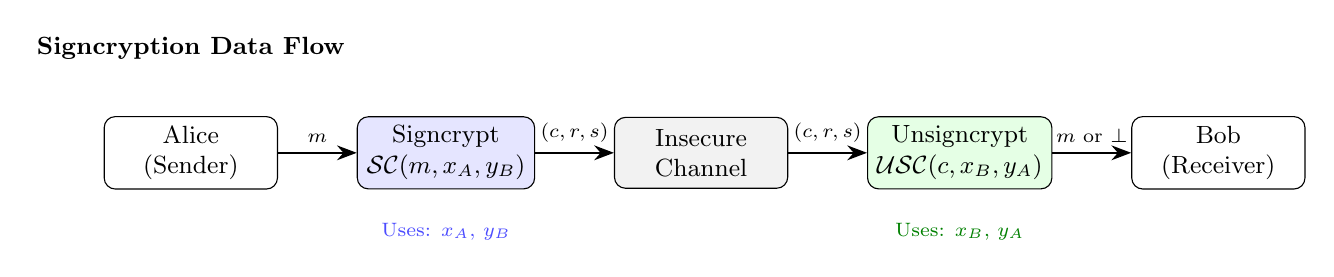
\begin{tikzpicture}[
    node distance=0.5cm and 0.6cm,
    box/.style={draw, rounded corners, minimum width=2.2cm, minimum height=0.9cm, font=\small, align=center},
    arrow/.style={-{Stealth[length=2.5mm]}, thick},
    label/.style={font=\small\bfseries}
]

% --- Signcryption Flow ---
\node[label] (title) {Signcryption Data Flow};

% Sender side
\node[box, below=0.6cm of title] (alice) {Alice\\(Sender)};
\node[box, right=1cm of alice, fill=blue!10] (sc) {Signcrypt\\$\mathcal{SC}(m, x_A, y_B)$};
\node[right=0.3cm of sc, font=\small] (inputs) {};

% Channel
\node[box, right=1cm of sc, fill=gray!10] (channel) {Insecure\\Channel};

% Receiver side
\node[box, right=1cm of channel, fill=green!10] (usc) {Unsigncrypt\\$\mathcal{USC}(c, x_B, y_A)$};
\node[box, right=1cm of usc] (bob) {Bob\\(Receiver)};

% Arrows
\draw[arrow] (alice) -- node[above, font=\scriptsize] {$m$} (sc);
\draw[arrow] (sc) -- node[above, font=\scriptsize] {$(c, r, s)$} (channel);
\draw[arrow] (channel) -- node[above, font=\scriptsize] {$(c, r, s)$} (usc);
\draw[arrow] (usc) -- node[above, font=\scriptsize] {$m$ or $\perp$} (bob);

% Keys
\node[below=0.3cm of sc, font=\scriptsize, text=blue!70] {Uses: $x_A$, $y_B$};
\node[below=0.3cm of usc, font=\scriptsize, text=green!50!black] {Uses: $x_B$, $y_A$};

\end{tikzpicture}
\caption{Data flow in a signcryption system. Alice signcrypts message $m$ using her private key $x_A$ and Bob's public key $y_B$. The signcrypted output $(c, r, s)$ is sent over an insecure channel. Bob unsigncrypts using his private key $x_B$ and Alice's public key $y_A$, recovering $m$ if verification succeeds or rejecting ($\perp$) otherwise.}
\label{fig:dataflow}
\end{figure}

% ============================================================
% TASK 3: Security Properties (5 Marks)
% ============================================================
\section{Task 3: Security Properties}

Signcryption achieves the following security properties simultaneously:

\subsection{Confidentiality}

Confidentiality ensures only the intended recipient can read the message. Signcryption achieves this through encryption using a key derived from the sender's ephemeral secret and the recipient's public key. Formally, this is captured as \textit{indistinguishability under adaptive chosen ciphertext attack} (IND-CCA2)---an adversary with decryption oracle access cannot distinguish between encryptions of two chosen plaintexts~\cite{baek2002}. In Zheng's scheme, confidentiality relies on the hardness of the Diffie--Hellman problem~\cite{zheng1997}.

\subsection{Integrity}

Integrity guarantees the message has not been altered during transmission. Signcryption ensures this through cryptographic binding between the message content and signature components---any modification causes unsigncryption verification to fail. Formally, integrity is captured as part of the unforgeability property~\cite{baek2002}.

\subsection{Authentication}

Authentication verifies the sender's identity. The sender's private key is an essential input to signcryption, and the recipient verifies identity using the sender's public key. This is formalized as \textit{existential unforgeability under adaptive chosen message attack} (EUF-CMA)---an adversary cannot forge a valid signcryption without the sender's private key~\cite{baek2002}. In Zheng's scheme, unforgeability reduces to the discrete logarithm problem.

\subsection{Non-repudiation}

Non-repudiation prevents the sender from denying having sent a message. The signature components can only be produced using the sender's private key, and a third-party judge can independently verify authorship~\cite{zheng1997}. Petersen and Michels~\cite{petersen1998} identified a subtle tension between non-repudiation and confidentiality in the original scheme, which was addressed in later constructions.

\subsection{Forward Secrecy}

Forward secrecy ensures that compromise of long-term keys does not expose past communications. Not all signcryption schemes provide this---Zheng's original does not. Boyen's identity-based scheme~\cite{boyen2003} achieves forward secrecy through ephemeral randomization: ephemeral keys independent of long-term keys are used and discarded, so past messages remain secure even if long-term keys are later compromised.

% ============================================================
% TASK 4: Comparative Analysis (8 Marks)
% ============================================================
\section{Task 4: Comparative Analysis of Selected Papers}

This section analyzes three seminal papers on signcryption, each representing a different stage in the evolution of the primitive.

\subsection{a) Summary of Selected Papers}

\subsubsection{Paper 1: Zheng (1997) --- ``Digital Signcryption''~\cite{zheng1997}}

\textbf{Objective:} Demonstrate that the cost of achieving both signature and encryption can be significantly less than their sum.
\textbf{Method:} Exploited common algebraic structure between ElGamal signatures and encryption, reusing the key exchange component for encryption. Operates over finite fields under DLP with 1536-bit moduli.
\textbf{Contribution:} Introduced signcryption, achieving 50\% computational savings (3 vs.\ 6 modular exponentiations) and 85\% communication savings. Defined the three required properties: unique unsigncryptability, security, and efficiency.

\subsubsection{Paper 2: Baek, Steinfeld, and Zheng (2002) --- ``Formal Proofs for Signcryption''~\cite{baek2002}}

\textbf{Objective:} Provide the first rigorous, reductionist security proofs for signcryption.
\textbf{Method:} Defined IND-CCA2 confidentiality and EUF-CMA unforgeability with signcryption/unsigncryption oracle access for the attacker.
\textbf{Contribution:} Proved Zheng's scheme secure in the random oracle model (confidentiality $\to$ GDH, unforgeability $\to$ DLP). Showed that encrypt-then-sign is completely insecure in the asymmetric setting.

\subsubsection{Paper 3: Boyen (2003) --- ``Multipurpose Identity-Based Signcryption''~\cite{boyen2003}}

\textbf{Objective:} Construct an identity-based signcryption with comprehensive security properties beyond basic confidentiality/unforgeability.
\textbf{Method:} Bilinear pairings under BDH assumption. Two-layer design: detachable randomized signature + anonymous deterministic encryption.
\textbf{Contribution:} Achieved IND-CCA2, EUF-CMA, ciphertext anonymity, unlinkability, authentication, and forward secrecy. Supports multi-recipient encryption with signature sharing.

\subsection{b) Comparative Analysis}

\textbf{Cryptographic Techniques:} Zheng uses DLP-based ElGamal over finite fields. Baek et al.\ formalize the same construction with GDH/DLP reductions. Boyen transitions to identity-based cryptography using bilinear pairings (BDH), eliminating certificate infrastructure.

\textbf{Computational Efficiency:} Zheng is the most efficient (3 mod.\ exp.\ for SC, 1 for USC). Baek et al.\ preserve this efficiency. Boyen's pairing operations are costlier, but eliminating certificate management reduces overall system overhead.

\textbf{Communication Overhead:} Zheng achieves 85\% reduction vs.\ StE. Baek et al.\ maintain the same. Boyen produces compact ciphertexts relative to separate IBE+IBS composition.

\textbf{Security Strength:} Zheng provides only informal arguments. Baek et al.\ give the first formal proofs (IND-CCA2, EUF-CMA) in ROM. Boyen offers the broadest guarantees: forward secrecy, ciphertext anonymity, and insider security.

\subsection{c) Comparison Table}

Table~\ref{tab:comparison} summarizes the comparative analysis across key dimensions.

\begin{table}[htbp]
\centering
\caption{Comparative Analysis of Selected Signcryption Schemes}
\label{tab:comparison}
\small
\begin{tabular}{@{}p{2.8cm}p{3.5cm}p{3.5cm}p{3.5cm}@{}}
\toprule
\textbf{Criterion} & \textbf{Zheng (1997)} & \textbf{Baek et al.\ (2002)} & \textbf{Boyen (2003)} \\
\midrule
\textbf{Setting} & PKI (finite field) & PKI (finite field) & Identity-based \\
\textbf{Crypto Technique} & DLP / ElGamal & GDH / DLP & BDH / Bilinear pairings \\
\textbf{Proof Model} & None (informal) & Random Oracle Model & Random Oracle Model \\
\textbf{Confidentiality} & Informal & IND-CCA2 & IND-CCA2 \\
\textbf{Unforgeability} & Informal & EUF-CMA & EUF-CMA \\
\textbf{Forward Secrecy} & No & No & Yes \\
\textbf{Ciphertext Anonymity} & No & No & Yes \\
\textbf{Comp.\ Cost (SC)} & 3 mod.\ exp. & 3 mod.\ exp. & Pairing operations \\
\textbf{Comm.\ Savings vs StE} & 85\% & 85\% & Compact (vs.\ IBE+IBS) \\
\textbf{Key Management} & Certificates (PKI) & Certificates (PKI) & Identity strings (no certs) \\
\textbf{Multi-recipient} & No & No & Yes \\
\bottomrule
\end{tabular}
\end{table}

% ============================================================
% TASK 5: Applications (3 Marks)
% ============================================================
\section{Task 5: Applications of Signcryption}

\subsection{Secure Email Systems}

Signcryption is naturally suited for secure email, where messages must be both confidential and authenticated. S/MIME and PGP currently use separate operations that could be replaced by signcryption. In the identity-based setting, email addresses serve directly as public keys, eliminating certificate management---historically the main barrier to encrypted email adoption~\cite{malonelee2002, boyen2003}.

\subsection{IoT Security}

IoT devices (wireless sensors, medical wearables, smart controllers) operate under severe computational, memory, and battery constraints. Signcryption's 50--58\% computational and 40--85\% communication savings are operationally decisive here. Recent work documents active adoption in IoT sensor networks, IoMT for health data, and VANETs for vehicle-to-infrastructure communication~\cite{iotsigncryption2025}. Elliptic curve signcryption~\cite{zheng1998} is particularly relevant due to ECC's shorter key sizes.

\subsection{Blockchain and Cryptocurrencies}

Blockchain transactions require both authentication and confidentiality. Signcryption reduces the cost of transaction signing and encryption, improving throughput. Identity-based signcryption suits permissioned blockchains where participant identities are known, enabling efficient authenticated communication without certificate infrastructure.

\subsection{E-Government and Financial Systems}

E-government services and financial systems require authenticated, confidential communication with non-repudiation. Signcryption provides all three in a single operation, reducing processing overhead. The non-repudiation property ensures legal accountability, while efficiency gains support high-throughput scalability.

% ============================================================
% TASK 6: Critical Evaluation (4 Marks)
% ============================================================
\section{Task 6: Critical Evaluation}

\subsection{a) Challenges and Limitations}

\begin{enumerate}[label=\arabic*.]
    \item \textbf{Post-quantum vulnerability:} All classical schemes rely on DLP, factoring, or pairings---vulnerable to Shor's algorithm. Lattice-based signcryption exists~\cite{sato2018} but practical post-quantum schemes with competitive performance remain under development.
    \item \textbf{Random oracle model dependence:} Every classical scheme with formal proofs relies on the ROM---an idealization that does not hold in practice~\cite{sato2018}.
    \item \textbf{Lack of library implementations:} No major cryptographic library implements signcryption natively, preventing practical evaluation by protocol designers.
    \item \textbf{Loss of modularity:} A monolithic primitive reduces algorithm agility---a vulnerability in one component forces replacing the entire scheme~\cite{an2002}.
    \item \textbf{Ecosystem inertia:} Hardware accelerators (AES-NI, ARM CryptoCell) have erased signcryption's efficiency advantage on equipped platforms.
    \item \textbf{Key escrow in IB settings:} The PKG can decrypt all messages and forge signatures. Certificateless signcryption~\cite{barbosa2008} mitigates this at the cost of analytical complexity.
\end{enumerate}

\subsection{b) Possible Improvements and Future Research Directions}

\begin{enumerate}[label=\arabic*.]
    \item \textbf{Post-quantum signcryption:} Efficient lattice/code-based schemes with competitive performance are the top priority. Sato--Shikata~\cite{sato2018} and G\'{e}rard--Merckx~\cite{gerard2018} provide foundations.
    \item \textbf{Standard-model proofs:} Classical schemes proven without random oracles would strengthen deployment confidence.
    \item \textbf{Reference implementations:} A conforming ISO/IEC 29150~\cite{iso29150} implementation in a major library (e.g., libsodium) would enable practical evaluation.
    \item \textbf{Protocol integration:} Proposals for integrating signcryption into TLS, DTLS, CoAP, or MQTT.
    \item \textbf{Pairing-free certificateless constructions:} Eliminating costly bilinear pairings for constrained IoT devices.
\end{enumerate}

\subsection{c) Overall Assessment}

Signcryption is a \textit{conditionally superior} alternative to traditional methods. For \textbf{resource-constrained environments} (IoT, IoMT, VANETs), it is clearly the better choice---50--58\% computational and 40--85\% communication savings are operationally decisive, explaining its active adoption in these domains. For \textbf{mainstream infrastructure} (TLS, Signal), advantages are largely neutralized by hardware acceleration and the practical benefits of modularity.

From a \textbf{security perspective}, signcryption offers genuinely different guarantees: the surreptitious forwarding attack against EtS~\cite{baek2002} and Badertscher et al.'s insider security analysis~\cite{badertscher2018} demonstrate it is a distinct primitive, not merely an optimization. Signcryption is theoretically sound, formally proven, and ISO-standardized. Its limited mainstream adoption is an ecosystem challenge, not a technical one. The post-quantum transition presents an opportunity to design signcryption into next-generation protocols from the ground up.

% ============================================================
% CONCLUSION
% ============================================================
\section{Conclusion}

This report analyzed signcryption across six dimensions: concept and motivation, architecture, security properties, comparative analysis of three key schemes, applications, and critical evaluation. Signcryption has evolved from Zheng's 1997 informal construction to formally proven, ISO-standardized schemes across multiple algebraic settings, offering 50--58\% computational and 40--85\% communication savings. It provides comprehensive security---confidentiality, integrity, authentication, non-repudiation, and (in advanced schemes) forward secrecy---and is most valuable in resource-constrained environments where it is already seeing active deployment. The main barriers to broader adoption are engineering challenges, not fundamental limitations, and the post-quantum transition presents a key opportunity for wider integration.

% ============================================================
% REFERENCES
% ============================================================
\begin{thebibliography}{17}

\bibitem{zheng1997}
Y.~Zheng, ``Digital signcryption or how to achieve cost(signature \& encryption) $\ll$ cost(signature) + cost(encryption),'' in \textit{Advances in Cryptology --- CRYPTO '97} (Lecture Notes in Computer Science, vol.~1294), B.~S.~Kaliski~Jr., Ed.\hspace{1em}Berlin, Germany: Springer, 1997, pp.~165--179.

\bibitem{zheng1998}
Y.~Zheng and H.~Imai, ``How to construct efficient signcryption schemes on elliptic curves,'' \textit{Information Processing Letters}, vol.~68, no.~5, pp.~227--233, 1998.

\bibitem{steinfeld2000}
R.~Steinfeld and Y.~Zheng, ``A signcryption scheme based on integer factorization,'' in \textit{Information Security} (Lecture Notes in Computer Science, vol.~1975), J.~Pieprzyk, E.~Okamoto, and J.~Seberry, Eds.\hspace{1em}Berlin, Germany: Springer, 2000, pp.~308--322.

\bibitem{baek2002}
J.~Baek, R.~Steinfeld, and Y.~Zheng, ``Formal proofs for the security of signcryption,'' in \textit{Public Key Cryptography --- PKC 2002} (Lecture Notes in Computer Science, vol.~2274), D.~Naccache and P.~Paillier, Eds.\hspace{1em}Berlin, Germany: Springer, 2002, pp.~80--98.

\bibitem{an2002}
J.~H.~An, Y.~Dodis, and T.~Rabin, ``On the security of joint signature and encryption,'' in \textit{Advances in Cryptology --- EUROCRYPT 2002} (Lecture Notes in Computer Science, vol.~2332), L.~R.~Knudsen, Ed.\hspace{1em}Berlin, Germany: Springer, 2002, pp.~83--107.

\bibitem{malonelee2002}
J.~Malone-Lee, ``Identity-based signcryption,'' \textit{Cryptology ePrint Archive}, Report 2002/098, 2002.

\bibitem{boyen2003}
X.~Boyen, ``Multipurpose identity-based signcryption: A Swiss army knife for identity-based cryptography,'' in \textit{Advances in Cryptology --- CRYPTO 2003} (Lecture Notes in Computer Science, vol.~2729), D.~Boneh, Ed.\hspace{1em}Berlin, Germany: Springer, 2003, pp.~383--399.

\bibitem{baek2007}
J.~Baek, R.~Steinfeld, and Y.~Zheng, ``Formal proofs for the security of signcryption,'' \textit{Journal of Cryptology}, vol.~20, no.~2, pp.~203--235, 2007.

\bibitem{iso29150}
ISO/IEC 29150:2011, ``Information technology --- Security techniques --- Signcryption,'' International Organization for Standardization, Geneva, Switzerland, 2011.

\bibitem{boneh2001}
D.~Boneh and M.~Franklin, ``Identity-based encryption from the Weil pairing,'' in \textit{Advances in Cryptology --- CRYPTO 2001} (Lecture Notes in Computer Science, vol.~2139), J.~Kilian, Ed.\hspace{1em}Berlin, Germany: Springer, 2001, pp.~213--229.

\bibitem{libert2003}
B.~Libert and J.-J.~Quisquater, ``New identity based signcryption schemes from pairings,'' in \textit{Proc. IEEE Information Theory Workshop (ITW 2003)}, Paris, France, 2003, pp.~155--158.

\bibitem{barbosa2008}
M.~Barbosa and P.~Farshim, ``Certificateless signcryption,'' in \textit{Proc. ACM Symposium on Information, Computer and Communications Security (ASIACCS 2008)}, Tokyo, Japan, 2008, pp.~369--372.

\bibitem{sato2018}
S.~Sato and J.~Shikata, ``Lattice-based signcryption without random oracles,'' in \textit{Post-Quantum Cryptography (PQCrypto 2018)} (Lecture Notes in Computer Science, vol.~10786), T.~Lange and R.~Steinwandt, Eds.\hspace{1em}Cham, Switzerland: Springer, 2018, pp.~331--351.

\bibitem{iotsigncryption2025}
M.~Rahmani, A.~Nitaj, and M.~Ziane, ``IoT-friendly certificateless signcryption schemes: Introducing a provably secure scheme in ROM,'' \textit{Journal of Information Security and Applications}, vol.~89, article 103981, 2025.

\bibitem{petersen1998}
H.~Petersen and M.~Michels, ``Cryptanalysis and improvement of signcryption schemes,'' in \textit{IEE Proceedings --- Computers and Digital Techniques}, vol.~145, no.~2, pp.~149--151, 1998.

\bibitem{badertscher2018}
C.~Badertscher, F.~Banfi, and U.~Maurer, ``A constructive perspective on signcryption security,'' in \textit{Security and Cryptography for Networks --- SCN 2018} (Lecture Notes in Computer Science, vol.~11035), D.~Catalano and R.~De~Prisco, Eds.\hspace{1em}Cham, Switzerland: Springer, 2018, pp.~102--120.

\bibitem{gerard2018}
F.~G\'{e}rard and K.~Merckx, ``Post-quantum signcryption from lattice-based signatures,'' \textit{Cryptology ePrint Archive}, Report 2018/861, 2018.

\end{thebibliography}

\end{document}
